\documentclass[12pt]{article}

% --- Font and Typography Fixes ---
\usepackage[T1]{fontenc}    
\usepackage{lmodern}        
\usepackage{microtype}      

% --- Packages ---
\usepackage[utf8]{inputenc}
\usepackage[margin=1in]{geometry}
\usepackage{graphicx} 
\usepackage{hyperref} 
\usepackage{tabularx} 
\usepackage{titlesec} 

% --- Link Styling ---
\hypersetup{
    colorlinks=true,
    linkcolor=black,
    filecolor=magenta,      
    urlcolor=blue,
    pdftitle={Big Data Analysis Project Report},
}

\begin{document}

% --- Title Page ---
\begin{titlepage}
    \centering
    
    \includegraphics[width=0.4\textwidth]{./pngs/logo2.png} 
    \\[1.5cm]
    
    {\Large \textbf{Course:} Fundamentals of Big-Data Analytics} \\
    {\large \textbf{Course Code:} CSE476s} \\[2cm]
    
    {\Huge \textbf{Big Data Analysis Project Report}} \\[0.5cm]
    
    {\Large \textbf{Automotive Market Insights Platform}} \\[2.5cm]
    
    {\Large \textbf{Team Members}}\\[0.5cm]
    \large
    \renewcommand{\arraystretch}{1.2} 
    \begin{tabular}{ll}
        Ahmed Said Sayed & 2101546 \\
        Abdelrahman Sherif Hassan & 2100735 \\
        Fares Khalaf Salman Sultan & 2101371 \\
        Yousef Mahmoud Mohamed & 2100994 \\
        Abdelrahman Taha Mohamed & 2100464 \\
        AbdElRahman Ahmed Soliman & 2100883 \\
        Mahmoud Essam Noureldin & 2001393 \\
        Zeyad Anwar Hussein & 2101073 \\
        Omar Tamer Mohamed & 2100528 \\
    \end{tabular}
    
    \vfill
\end{titlepage}

\newpage
\tableofcontents
\newpage

% --- Main Document ---

\section{Problem Description}

The Egyptian automotive market, particularly the used car sector, is currently overwhelmed by a massive influx of unstructured and fragmented data scattered across online marketplaces. Buyers, sellers, and automotive dealerships alike face significant challenges in navigating this complex data landscape to make informed financial decisions.

For buyers, the sheer volume of listings and the reliance on free-form, unstructured Arabic text for vehicle descriptions make it exceedingly difficult to identify the true market value, condition, and detailed specifications of a car. Vital details such as paint condition (e.g., factory paint vs. repainted), specific trim levels, and exact feature sets are often buried within long paragraphs rather than standardized, easily searchable fields.

For dealerships and market analysts, monitoring competitor pricing, tracking brand popularity, and understanding the depreciation curves of specific models based on their condition is a highly labor-intensive process. The inability to systematically filter or analyze vehicles based on these "hidden" specifications leads to missed opportunities for dynamic pricing, inventory acquisition, and accurate market forecasting.

\textbf{Key issues include:}
\begin{itemize}
    \item \textbf{Information Overload:} Thousands of active vehicle listings across platforms like Hatla2ee make manual tracking, comparison, and verification practically impossible for the average consumer.
    \item \textbf{Unstructured Data Dependency:} Crucial vehicle specifications—such as engine capacity, drivetrain format, and paint condition—are locked within unstructured, often colloquial Arabic descriptions rather than accessible database columns.
    \item \textbf{Lack of Actionable Insights:} Raw listing data does not easily translate into clear market trends (e.g., pricing variations based strictly on paint condition or specific trim variants) without the application of sophisticated Natural Language Processing (NLP) and automated data extraction pipelines.
\end{itemize}

\newpage
\section{Business and Market Benefits}

The proposed Big Data Analytics Platform offers substantial value to both the B2C (Business-to-Consumer) and B2B (Business-to-Business) segments within the automotive sector. By transforming unstructured descriptions into actionable intelligence, the platform bridges the gap between vehicle condition and price perception.

\vspace{0.5cm}
\noindent
\renewcommand{\arraystretch}{1.5} 
\begin{tabularx}{\textwidth}{|>{\raggedright\arraybackslash}p{4.5cm}|X|}
    \hline
    \textbf{Stakeholder} & \textbf{Key Benefits} \\
    \hline
    \textbf{Car Buyers \newline (Consumers)} & Informed decision-making, time-saving in vehicle research, and direct access to high-value listings by filtering hidden specifications like factory paint condition, exact engine capacity, and trim levels. \\
    \hline
    \textbf{Dealerships \& Sellers \newline (B2B)} & Competitive intelligence, real-time market monitoring, and data-driven insights to optimize dynamic pricing and inventory acquisition based on accurate market trends and vehicle depreciation curves. \\
    \hline
    \textbf{Market Impact} & Increased market transparency and efficiency by standardizing colloquial Arabic descriptions into clear English metrics, creating a fairer marketplace where prices accurately reflect true vehicle conditions. \\
    \hline
\end{tabularx}

\newpage
\section{Technical Description}

The technical architecture of this project is structured into a three-stage Big Data pipeline: automated data acquisition, NoSQL database migration, and an AI-driven Natural Language Processing (NLP) enrichment phase.

\subsection{Data Acquisition (Web Scraping Phase)}
The initial phase involved extracting raw vehicle listings from the Hatla2ee platform. A robust Python scraper was developed utilizing the \textbf{BeautifulSoup} library for HTML parsing alongside \textbf{cloudscraper} to bypass advanced Cloudflare anti-bot protections.
\begin{itemize}
    \item \textbf{Scope and Scale:} The scraper was configured to target 15 major automotive brands, iterating through up to 51 pagination levels per brand to ensure maximum market coverage.
    \item \textbf{Resiliency and Session Management:} To prevent IP bans and ensure uninterrupted extraction, the script implemented exponential backoff retry mechanisms, HTTP session pooling, and randomized jitter delays to simulate natural human browsing behavior.
    \item \textbf{Data Capture:} Beyond scraping basic tabular data (e.g., brand, model, year, price, transmission), the scraper executed secondary requests to individual vehicle pages to capture the full, unstructured Arabic text descriptions. While this synchronous approach ensured high-fidelity data capture, it intentionally prioritized data depth over scraping speed, introducing a known processing bottleneck due to the sheer volume of network requests. This initial raw dataset was stored in a temporary CSV file.
\end{itemize}

\newpage
\subsection{Data Storage and Migration}
To accommodate the unstructured nature of the Arabic text descriptions and the dynamic schema of the subsequent AI-extracted features, the data architecture transitioned from a flat-file CSV model to a NoSQL document database.
\begin{itemize}
    \item \textbf{Migration Pipeline:} A Python pipeline leveraging \textbf{Pandas} for data ingestion and formatting, alongside \textbf{PyMongo} for database connectivity, was built to efficiently read the CSV data and batch-insert it into \textbf{MongoDB}.
    \item \textbf{Architectural Rationale:} MongoDB was explicitly chosen for its flexibility in handling deeply nested JSON objects, making it the ideal storage solution for the dynamically generated arrays and key-value pairs produced by the Generative AI model in the next phase.
\end{itemize}

\subsection{Intelligent Data Processing Pipeline}
The core analytical innovation of this project lies in transforming colloquial Egyptian Arabic descriptions into structured, queryable data fields using Generative AI.
\begin{itemize}
    \item \textbf{LLM Integration:} The pipeline utilized \textbf{LangChain} to orchestrate prompts and connected to a Generative AI model (\textbf{Gemma}) via the Google Generative AI API. The model's temperature was strictly set to 0.2 to ensure high determinism and eliminate hallucinations during data extraction.
    \item \textbf{Feature Engineering \& Label Creation:} Using the \textbf{Pydantic} library, a strict schema was enforced. The LLM acted as an automated feature engineering tool, reading the unstructured Arabic descriptions to generate entirely new, structured data labels for each car. It successfully created new database columns for metrics that were previously hidden, including exact engine capacity (CC), horsepower, drivetrain configuration (e.g., 4WD, FWD), specific trim levels, and critical valuation metrics like paint condition.
    \item \textbf{Translation \& Standardization:} The prompt instructions required the model to translate localized Arabic automotive jargon and feature lists into standardized English arrays, unifying the dataset for analysis.
    \item \textbf{Batch Processing:} The pipeline fetched documents from MongoDB, processed the unstructured text through the LLM via concurrent batches to handle API rate limits, and directly wrote the enriched JSON data back into the database using bulk update operations.
\end{itemize}

\newpage
\section{Results}

The culmination of the web scraping and AI-driven data extraction pipeline resulted in a highly structured, queryable database of the Egyptian used car market. To extract meaningful insights, the data underwent a final cleaning phase before being visualized through business intelligence dashboards.

\subsection{Data Cleaning and Preprocessing}
Before visualization, the raw dataset required numerical standardization. Critical valuation fields such as \texttt{price} and \texttt{mileage} were initially scraped as formatted strings (e.g., "1,350,000" and "85,000 KM"). To enable accurate mathematical operations, we executed \textbf{MongoDB update queries} utilizing regex and aggregation pipelines to strip non-numeric characters (commas, text suffixes) and cast these fields into pure integer data types. This transition from string to integer types was essential for calculating averages, plotting scatter distributions, and generating accurate market trends.

\subsection{Exploratory Data Analysis \& Market Insights}

With the data cleaned and the hidden Arabic specifications successfully translated and extracted by the Gemini LLM, we generated several key visualizations to map the automotive market on Hatla2ee.

\vspace{0.3cm}
\noindent\textbf{1. Market Volume vs. Average Price (By Brand)} \\
Our analysis compared the volume of listings against the average price across major brands. The data reveals that luxury brands like Mercedes hold the highest average valuation, while brands like Hyundai, Kia, and BMW dominate the market in sheer listing volume, indicating high liquidity and popularity in the Egyptian market.

\begin{figure}[h]
    \centering
    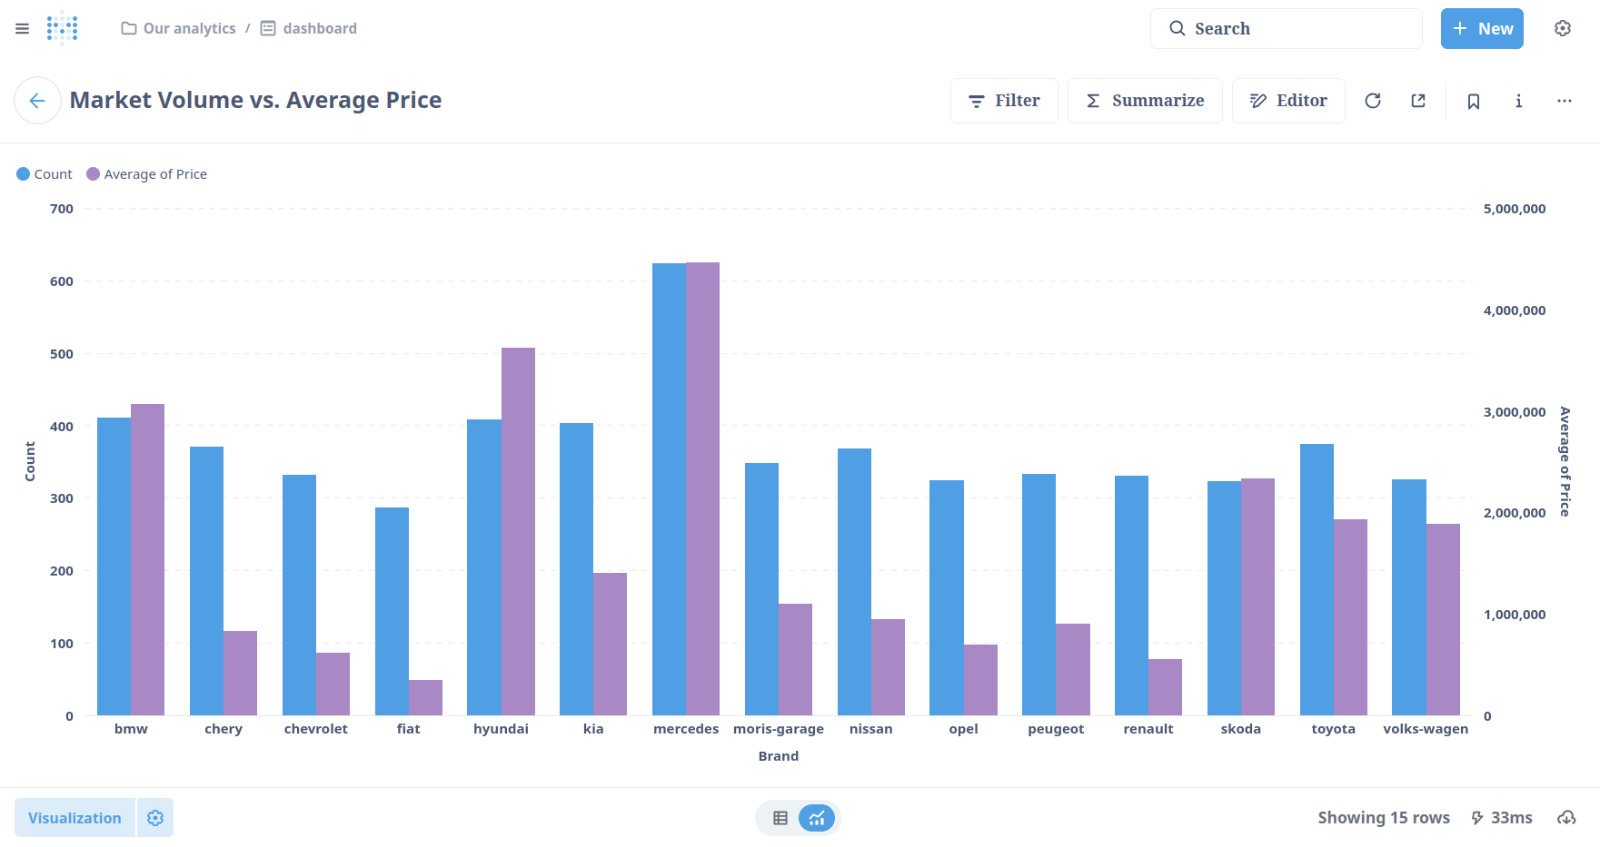
\includegraphics[width=1.0\textwidth]{./pngs/mv_vs_avP.jpeg} 
    \caption{Analysis of Market Volume  vs. Average Vehicle Price per Brand }
\end{figure}

\subsubsection*{Market Insight: Brand Dominance and Price Distribution}

By aggregating the data across the fifteen most prominent brands on \textbf{Hatla2ee}, a clear correlation emerges between brand reputation and market activity. 

\begin{itemize}
    \item \textbf{High-Value Market Leader:} Mercedes stands out as the dominant brand, exhibiting both the highest listing volume and the highest average price, indicating a uniquely strong presence in the premium segment of the Egyptian used car market.
    \item \textbf{Mid-Range Liquidity:} Brands like \textbf{Hyundai, Kia, and BMW} show high market volume with significant price averages, representing the "sweet spot" of the Egyptian used car market where high demand meets substantial capital investment.
    \item \textbf{Economy Segment:} \textbf{Fiat and Renault} represent the high-liquidity budget segment, showing healthy listing counts but maintaining the lowest average price points. This data allows for clear market segmentation, separating luxury tiers from high-volume economy options for better targeted analysis.
\end{itemize}

\vspace{0.3cm}
\noindent\textbf{2. Average Price per Year} \\
The historical pricing trend shows relatively stable and low valuations for vehicles manufactured before 2010. However, there is a massive exponential spike in average prices for models manufactured after 2018, reflecting severe recent market inflation, currency devaluation impacts, and the high premium placed on modern features.

\begin{figure}[h]
    \centering
    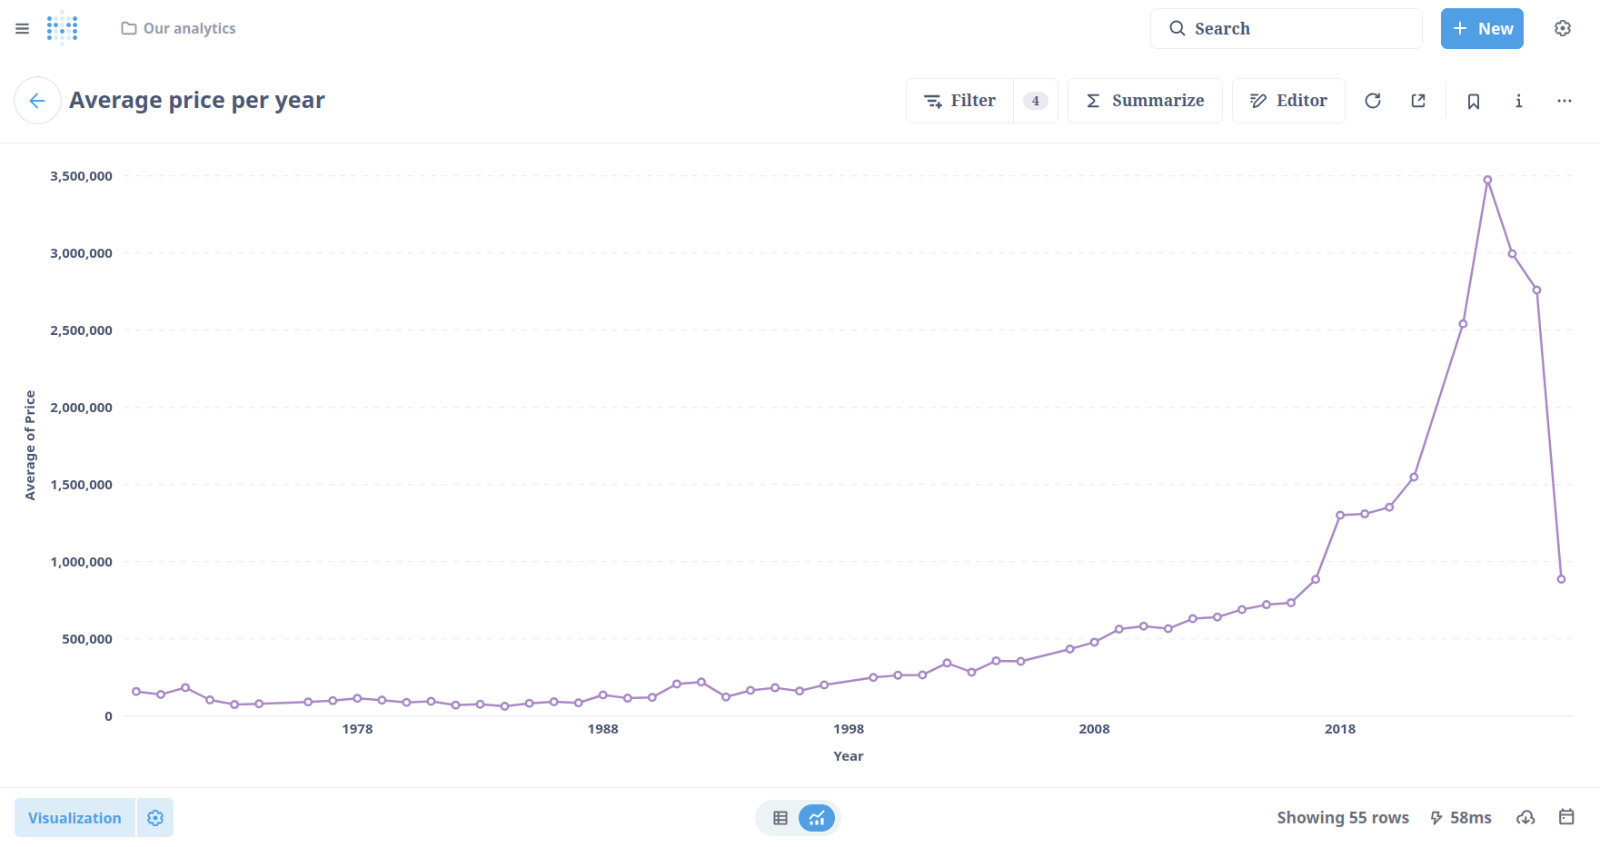
\includegraphics[width=1.0\textwidth]{./pngs/avgPY.jpeg} 
    \caption{Chronological Trend of Average Vehicle Prices  }
\end{figure}

\subsubsection*{Market Insight: The Chronological Price Explosion}

The line chart tracking average vehicle prices across nearly six decades reveals a stark narrative of market volatility and economic shifts in the Egyptian automotive sector.

\begin{itemize}
    \item \textbf{Historical Stability (1970--2010):} For nearly forty years, the average price of used vehicles remained relatively flat and predictable. During this period, cars were treated as long-term assets with slow depreciation and minimal price fluctuations.
    \item \textbf{The Post-2018 Inflection Point:} A dramatic exponential spike is observed starting around 2018. The average price surged from approximately 1,000,000 EGP to a peak of nearly 3,500,000 EGP by 2024. This trend highlights the severe impact of local currency devaluation, high inflation rates, and the significant premium placed on modern "Zero" or "Near-Zero" models.
    \item \textbf{Modern Premium vs. Classic Value:} The data demonstrates that vehicles manufactured in the last five years carry a disproportionately higher market value compared to the preceding four decades combined. This insight is crucial for dealerships for predictive pricing and for consumers to understand the rapid "aging out" of purchasing power in the current market climate.
\end{itemize}


\vspace{0.3cm}
\noindent\textbf{3. Mileage vs. Price categorized by brand} \\
By plotting mileage against price, we established a clear market depreciation curve. The scatter plot demonstrates a steep initial drop in price as a vehicle moves from "Zero" kilometers to 100,000 KM, after which the depreciation curve flattens out. Luxury vehicles (e.g., Mercedes, BMW) show a wider variance in price retention compared to economy brands.

\begin{figure}[h]
    \centering
    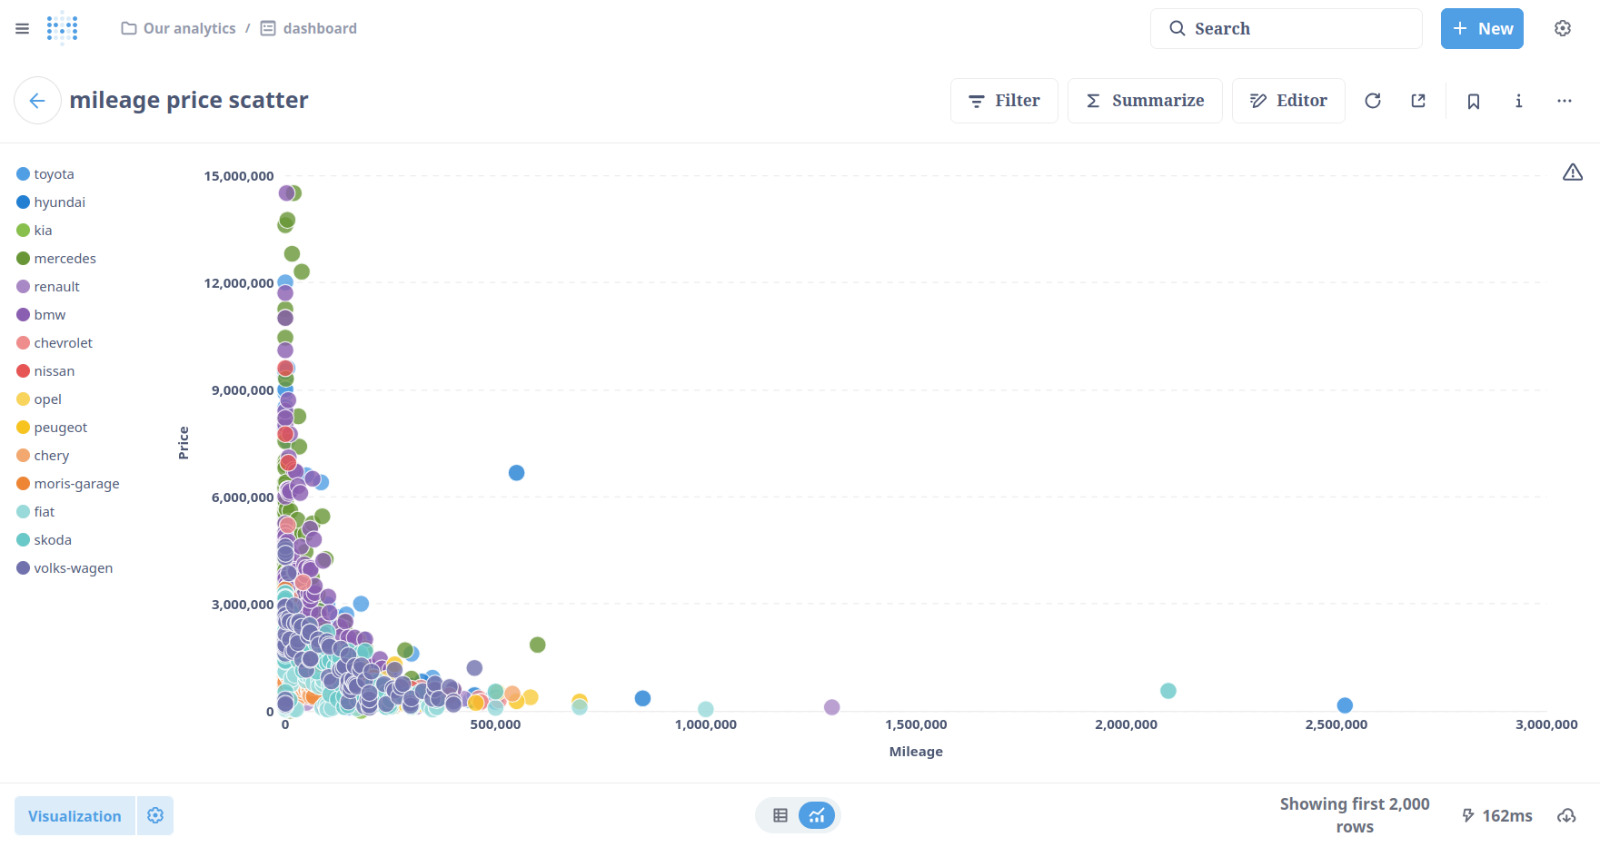
\includegraphics[width=1.0\textwidth]{./pngs/mileage_scatter.jpeg} 
    \caption{Scatter Plot of Mileage vs. Price categorized by brand}
\end{figure}

\subsubsection*{Market Insight: The Non-Linear Depreciation Curve}

The scatter plot of mileage versus price establishes a definitive "L-curve" depreciation model for the Egyptian automotive market.

\begin{itemize}
    \item \textbf{The "Zero" Kilometer Premium:} There is a massive vertical cluster at the 0--5,000 KM mark. In this "Zero" or "Near-Zero" zone, prices reach their absolute peak, often exceeding 12,000,000 EGP for luxury brands. The data shows that the mere transition from a "Zero" status to a used status triggers the most significant single drop in vehicle valuation.
    \item \textbf{Brand-Based Price Dispersion:} At lower mileage ranges, luxury brands such as Mercedes and BMW exhibit a significantly wider spread in price compared to economy brands. This suggests that factors beyond mileage—such as trim level, features, and condition—play a larger role in determining value within the premium segment.
    \item \textbf{High-Mileage Convergence:} As mileage exceeds 500,000 KM, the price variance between different brands begins to converge. Regardless of the initial brand prestige, vehicles with extremely high mileage tend to stabilize at a lower market "floor" price. Additionally, a small number of extreme high-mileage outliers (exceeding 1,000,000 KM) are observed, which likely represent data anomalies or entry inconsistencies rather than typical market behavior.
    \item \textbf{AI-Powered Granularity:} As shown in the data tooltip, the platform does not just plot raw numbers; it integrates \textbf{AI-extracted qualitative data}. For instance, the system can identify a 2018 Volkswagen priced at 1,270,000 EGP and immediately provide context extracted from the original description.
\end{itemize}

\vspace{0.3cm}
\noindent\textbf{4. Valuation by Paint Condition } \\
This metric highlights the success of the NLP pipeline. By grouping average prices based on the AI-extracted "Paint Condition", the visualization reveals significant variation in average price across different paint condition categories. This demonstrates that unstructured text holds direct, quantifiable financial value in the automotive market.
\begin{figure}[h]
    \centering
    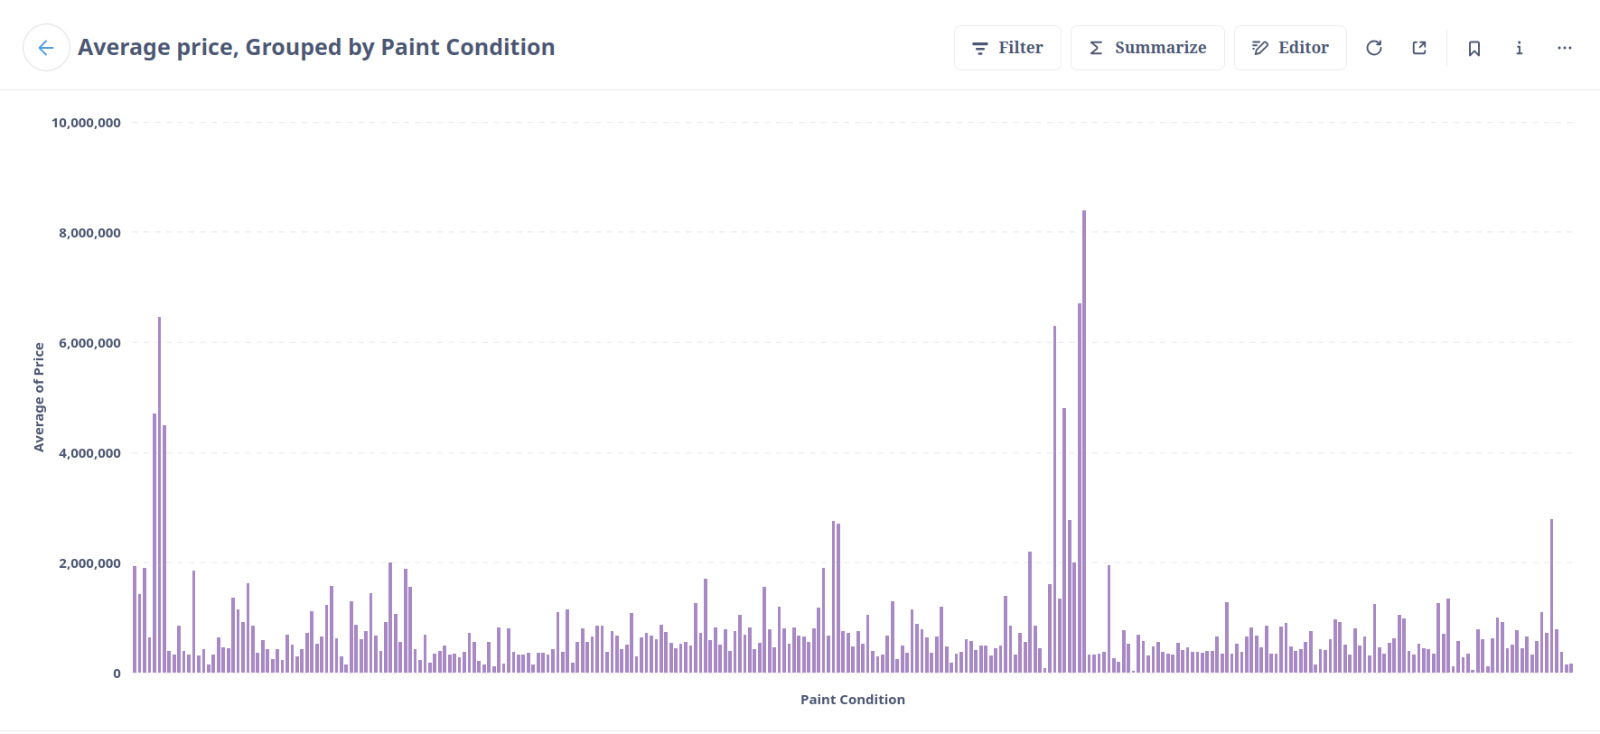
\includegraphics[width=1.0\textwidth]{./pngs/paint_condition.jpeg} 
    \caption{Average Vehicle Price Grouped by Extracted Paint Condition Metrics.}
\end{figure}

\subsubsection*{Market Insight: The High Premium of Originality}

This visualization represents the most significant outcome of the \textbf{AI-driven enrichment phase}, indicating that qualitative data extracted from unstructured text has a direct, quantifiable impact on vehicle valuation.

\begin{itemize}
    \item \textbf{The "Original Paint" Spike:} While the distribution is fragmented due to diverse seller descriptions, clear price spikes indicate that specific high-quality conditions command a substantial premium. These spikes correspond to labels indicating original factory conditions. In the Egyptian market, vehicles maintaining their original factory finish often command a significantly higher market value compared to models with a repainted exterior.
    \item \textbf{Standardizing Colloquialisms:} The horizontal axis displays a wide variety of conditions parsed from the Hatla2ee descriptions. Our AI pipeline successfully categorized these from diverse seller phrasing (e.g., \textit{"partial repaint"}, \textit{"beltline repaint"}), allowing for the first time a systematic comparison of how "clean" or "partial" repaints affect the bottom-line price compared to total factory condition.
    \item \textbf{Actionable Value for Stakeholders:} By standardizing these conditions into a queryable format, a consumer can now mathematically verify the "fair price" for a car based on its aesthetic history. For dealerships, this data indicates that investing in vehicles with original paint—even at a higher acquisition cost—is a more profitable strategy due to the disproportionately high resale value and market demand for "untouched" units.
\end{itemize}

\newpage
\section{Project Links}

\textbf{Public Google Drive Link (Data, Code, Demo Video):} \\
\url{https://drive.google.com/your-public-link-here}

\end{document}